\documentclass[a4paper,10pt]{article}
\usepackage{amsmath}
\usepackage[italian]{babel}
\usepackage[utf8]{inputenc}
\usepackage{graphicx}

\begin{document}

\title{Report - Secondo assegnamento Ingegneria del Software}
\author{Vincenzo Arceri - VR360465\\
 Matteo Calabria - VR363871\\
 Pietro Musoni - VR359914\\ 
Carlo Tacchella - VR362194\\}
\date{Anno accademico 2013/2014}
\maketitle

\section{Specifiche del progetto}

L' \textit{Automotive System} è un esempio di sistema per connettere tramite rete wireless automobili su un tratto stradale ad una base centrale per il controllo delle velocità e del traffico. Il sistema è composto da tre nodi principali: i canali, la stazione e le automobili. La stazione invia i pacchetti per la comunicazione in broadcast a tutte le auto sul tratto coperto dalla rete, queste rispondono direttamente alla stazione e qualora ci fossero posti disponibili sui canali controllati dalla stazione vengono registrate su uno di essi. I canali possono essere al massimo cinque e hanno una capacità uguale a 100 pps. Una volta raggiunto il limite di auto connesse il canale non può ospitarne altre e sarà creato un ulteriore canale fino al raggiungimento del limite consentito (cinque canali).   
Lo scenario è quindi il seguente:
\begin{itemize}
\item la stazione gestisce il sistema di registrazione delle auto e comunica in broadcast con le auto connesse al sistema per il controllo della velocità;
\item i canali collegano la automobili registrate con la stazione e controllano il flusso di informazioni che queste inviano alla stazione;
\item le automobili possono essere di due tipi (automatiche o manuali) e in base al loro tipo reagiscono in modi differenti ai messaggi della stazione per quanto riguarda l'adeguamento dei limiti di velocità. 
\end{itemize}


\section{Scelte progettuali}
Il diagramma delle classi riporta lo schema del progetto, mostrando graficamente le scelte implementative, le assunzioni ed i pattern utilizzati (Figura 1). Il sistema è principalmente composto da tre oggetti che comunicano fra di loro; la stazione e l'auto sono dei nodi ed estendono rispettivamente la classe \textit{Node} e la classe \textit{AbstractCar}, che estende a sua volta la classe Node. Un possibile scenario di applicazione è il seguente: la stazione ha la referenza di ogni auto creata e inizialmente la stazione inviterà tutte le auto a registrarsi ad un canale; le auto risponderanno alla stazione riportando il proprio tipo e identificativo: la stazione controllerà i canali attivi fino a quel momento e se ne trova uno libero registra l'auto su quel canale altrimenti, se tutti i canali creati sono occupati, tenterà di crearne uno nuovo; raggiunto il limite di possibili canali ritornerà semplicemente un messaggio che indica che tutti i canali sono pieni.

Una volta che l'auto è registrata nel sistema, invierà periodicamente (in base al proprio packet rate) la propria velocità alla stazione tramite il canale che funge da dispatcher fra le auto e la stazione base. La stazione base controllerà i messaggi ogni secondo, in base al proprio packet rate, ed invierà gli opportuni messaggi alle auto che alla ricezione visualizzeranno sul proprio display; alle auto che superano la velocità limite indicata dalla threshold invierà un messaggio che le invita a rallentare, altrimenti un messaggio positivo. Nel caso di auto automatiche che superano il limite  diminuiranno automaticamente la velocità fino a 49 Km/h,tramite la funzione \textit{breaking},  altrimenti continueranno a modificare la propria velocità casualmente come le auto manuali indipendentemente dal tipo di messaggio ricevuto dalla stazione.

Il formato dei messaggi è modellato dalla classe Packet, la cui implementazione è conosciuta dalle auto e dalla stazione.

L'azione periodica di invio dei messaggi è gestita tramite un TimerTask, che scandisce l'azione che deve essere ripetuta periodicamente, in base al packet rate di ogni nodo.

Ogni 12 secondi la stazione genererà due identificativi di auto e, se validi, le deregistrerà dal sistema, impedendogli di registrarsi in un secondo momento; successivamente invierà in broadcast un nuovo messaggio per invitare le auto eventualmente non ancora registrate ad entrare nel sistema.

Le macchine vengono generate casualmente dalla classe FactoryCar, che genera 90 auto. 
%%%%%%%


\begin{figure}[htbp]
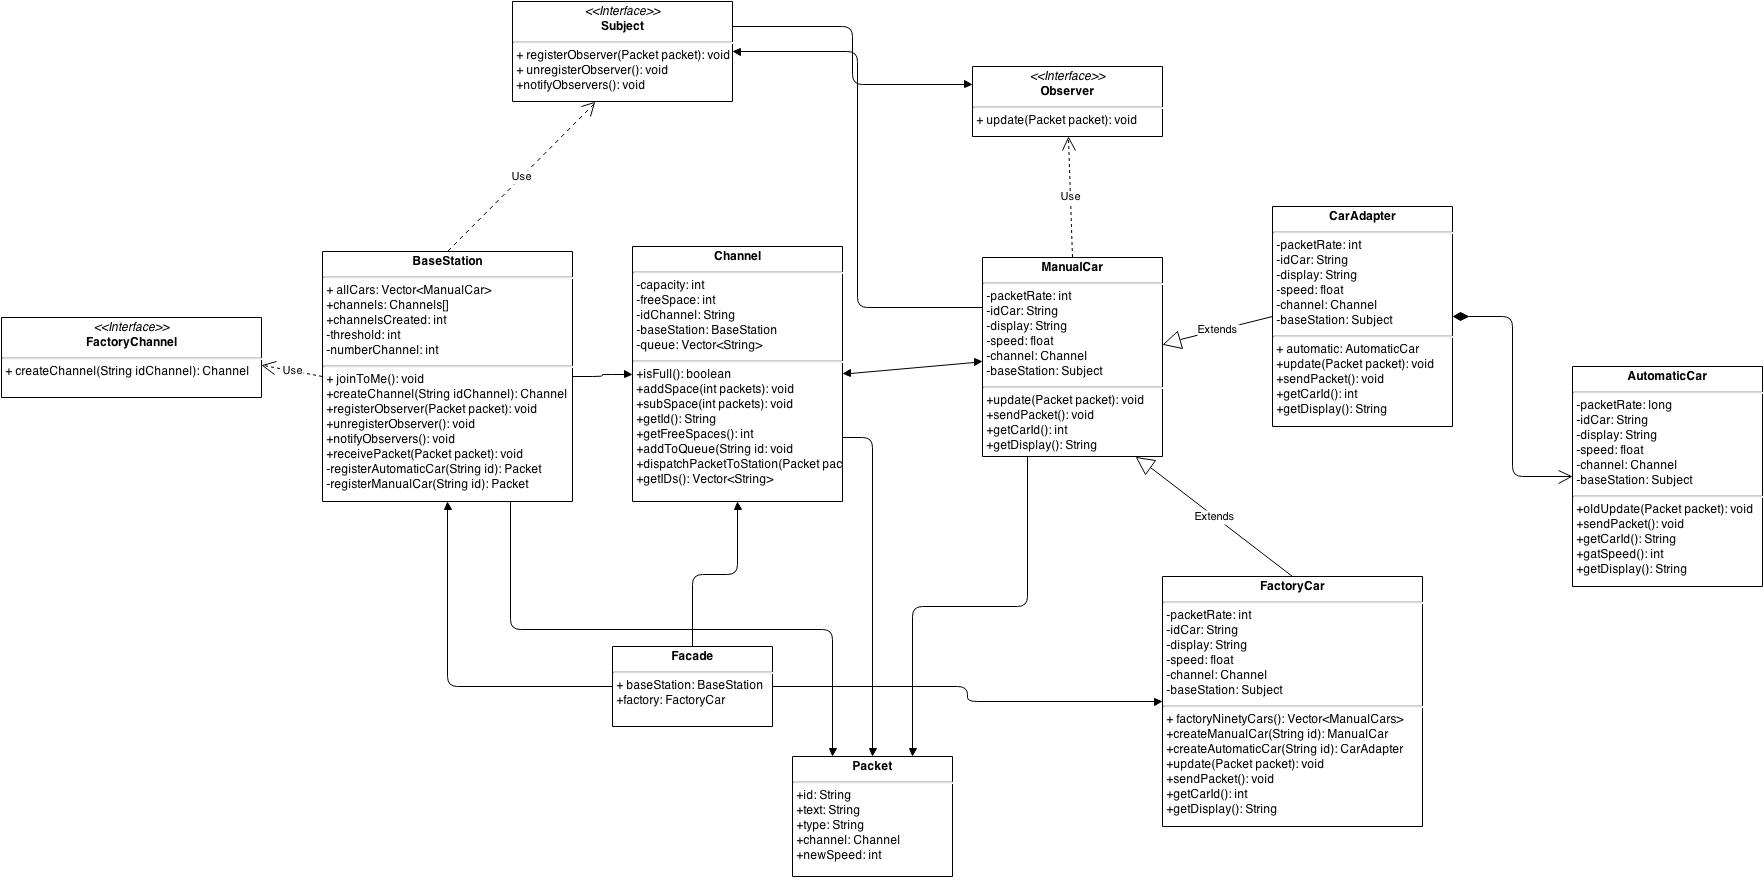
\includegraphics[scale=0.24]{class_diagram.jpg}
\caption{Diagramma delle classi}
\label{class_dig}
\end{figure}


La classe Facade crea la base station e il factory car per inizializzare il sistema, il facade viene creato invece dal main di Simulator che implementa anche la parte grafica composta da due finestre.
Una tabella presenta la velocità, il display e l'id di tutte le automobili registrate ai canali mentre l'altra finestra segnala lo stato di ogni canale scrivendo la percentuale di occupazione. Dato che ogni canale riesce a reggere al massimo un packet rate di 100 pps, se si registra un auto manuale vengono occupati 5 pps, se se ne registra una automatica se ne occupano 10 (come da specifiche). 
Se un'auto si deregistra vengono liberati i rispettivi pps dal flusso del canale permettendo così la registrazione di nuove vetture al canale.
Quando un'auto invia la velocità alla base station, sul display viene scritto che l'auto in questione sta aspettando una risposta. 

\section{Design pattern utilizzati}

La stazione centrale ha un'interfaccia \textbf{FactoryChannel} per la creazione dei canali e un'interfaccia \textbf{Subject} per l'invio di pacchetti a tutte le auto tramite il metodo \textbf{update} dell'interfaccia \textbf{Observer} (come specificato dall' omonimo design pattern). 

Ogni auto è estesa da una classe \textbf{Adapter} per adattare le automobili manuali ad automibili automatiche, cambiando il metodo update che nel secondo caso, invece di mostrare semplicemente un messaggio su display, chiama automaticamente il metodo \textbf{break} che fa frenare l'auto in questione. Ogni auto viene creata da una classe \textbf{FactoryCar}. Se un'auto riesce a registrarsi su un canale, comunica tramite quest'ultimo con la base station, mentre tutti i pacchetti che partono dalla stazione vengono inviati direttamente alle auto in broadcast. I pacchetti sono definiti dalla classe \textbf{Packet}, che ne descrive i campi.
I pattern implementati richiesti dalle specifiche sono: Facade e Adapter. Il primo è utilizzato per visualizzare lo stato di tutti i nodi, usati per l'interfaccia con l'utente. Il pattern Adapter viene utilizzato per adattare le auto automatiche in auto manuali, poiché differiscono solamente nel metodo update (come visto in precedenza, per le automatiche si chiama il metodo break in caso di messaggio di rallentamento mentre le altre stampano solo un messaggio sul display). 

I design pattern che abbiamo deciso di implementare sono: Observer e Factory. Il modello Observer permette la comunicazione diretta tra la base station e le automobili, inizialmente in entrambe le direzioni per gestire la registrazione delle auto sul canale, in seguito a una direzione ovvero dalla base station alle auto per l'invio in broadcast dei pacchetti di comunicazione (canale pieno, rallenta etc..).

Il primo scenario in cui viene applicato il pattern factory è per creare le automobili che possono essere manuali o automatiche. Il secondo scenario in cui è utilizzato è per la creazione dei canali da parte della stazione centrale.

\end{document}
